\newcommand{\fcaclusterconnection}{%
\begin{figure}[h]
\centering
\caption{Similarities between FCA and constrained clustering.
Similarity-based is 2D representation, where dimensions are not explicitely interpretable (unlike with object-attribute description). Distances in this space have a semantic meaning.}
\label{fig:fcaclusterconnection}
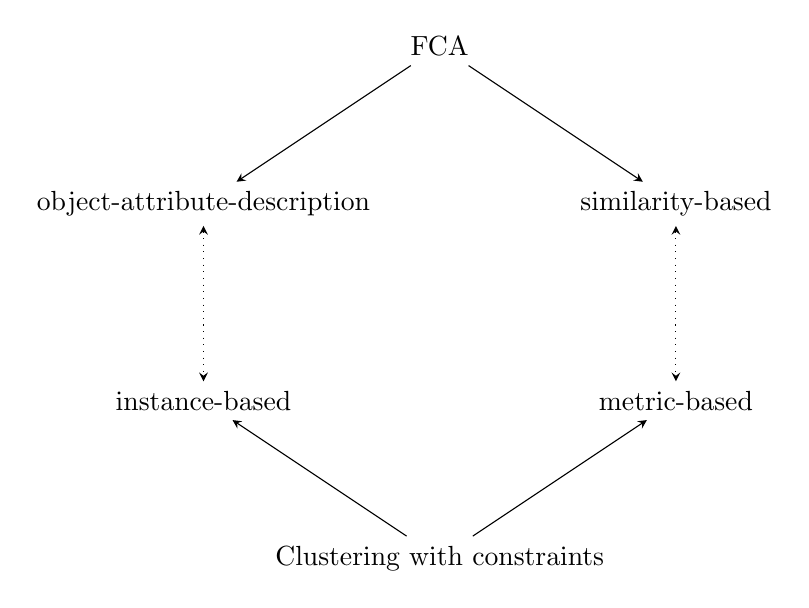
\begin{tikzpicture}[>=stealth]

% Nodes (placed manually to avoid positioning errors)
\node (FCA) at (0,0) {FCA};

\node (OAD) at (-3,-2) {object-attribute-description};
\node (SIM) at (3,-2) {similarity-based};

\node (CWC) at (0,-6.5) {Clustering with constraints};

\node (IB) at (-3,-4.5) {instance-based};
\node (MB) at (3,-4.5) {metric-based};

% Directed arrows
\draw[->] (FCA) -- (OAD);
\draw[->] (FCA) -- (SIM);

\draw[->] (CWC) -- (IB);
\draw[->] (CWC) -- (MB);

% Bidirectional arrows
\draw[<->, dotted] (OAD) -- (IB);
\draw[<->, dotted] (SIM) -- (MB);

\end{tikzpicture}

\end{figure}
}
